\documentclass{article}
\PassOptionsToPackage{numbers, compress}{natbib}
\usepackage[dblblindworkshop]{neurips_2026}
\workshoptitle{TAE (Trust-AI-Eval): Can We Trust AI Evaluation?}

\usepackage[utf8]{inputenc}
\usepackage[T1]{fontenc}
\usepackage{hyperref}
\hypersetup{hidelinks}
\usepackage{url}
\usepackage{booktabs}
\usepackage{amsfonts}
\usepackage{amsmath, amssymb}
\usepackage{nicefrac}
\usepackage{microtype}
\usepackage{xcolor}
\usepackage{multirow}
\usepackage{float}
\usepackage{tikz}
\usetikzlibrary{shapes.geometric, arrows.meta, positioning, fit, backgrounds}

\tikzset{
  mainbox/.style={rectangle, rounded corners=4pt, minimum width=8cm, minimum height=1.0cm,
    text centered, text width=7.8cm, font=\small\bfseries, inner sep=6pt},
  navybox/.style={mainbox, fill=blue!25!black, text=white},
  bluebox/.style={mainbox, fill=blue!55, text=white},
  lightbox/.style={mainbox, fill=blue!10, text=blue!30!black, draw=blue!40, line width=0.8pt},
  greenbox/.style={mainbox, fill=green!35!black, text=white},
  brownbox/.style={mainbox, fill=orange!40!brown, text=white},
  warmbox/.style={mainbox, fill=orange!15, text=orange!40!brown, draw=orange!40!brown, line width=0.8pt},
  purplebox/.style={mainbox, fill=violet!60!black, text=white},
  clusterbox/.style={rectangle, rounded corners=3pt, minimum width=2.3cm, minimum height=0.9cm,
    text centered, text width=2.1cm, font=\small\bfseries, fill=green!15, draw=green!40!black,
    line width=0.8pt, text=green!30!black},
  arrow/.style={-Stealth, thick, blue!40!black}
}

\title{Peer-Isolated Recommendation: When Content-Only Personalization Beats Collaborative Signal, and When It Doesn't\footnotemark}

\author{%
  Anonymous Author(s) \\
  Affiliation \\
  Address \\
  \texttt{email}
}

\begin{document}

\maketitle
\footnotetext{Code and data: \url{https://anonymous.4open.science/r/essence-5B7B/README.md}}

\begin{abstract}
We present Essence, a personal embedding cluster framework for recommendation that operates exclusively within a single user's engagement history, without consulting cross-user interaction data. We evaluate Essence on three datasets spanning music, e-commerce, and film (Last.fm-1K, Amazon Books, MovieLens-25M) against nine baselines, including collaborative filtering, popularity, recency-based retrieval, and two hand-implemented multi-interest neural baselines (MIND, ComiRec), with $K$ selected per dataset on a validation split rather than fixed in advance ($K=10$ Last.fm-1K/Amazon Books, $K=15$ MovieLens-25M). Across these three datasets, Essence's relative standing is associated with observed collaborative-baseline strength; establishing this as predictive would require additional datasets and an independently-defined domain property. Where the evaluated collaborative baselines perform weakly, Essence ranks 2nd of 10 on Last.fm-1K and 3rd on Amazon Books, significantly beating collaborative filtering, popularity, and both neural baselines, and not significantly different from most recency-only baselines; where they perform strongly (MovieLens-25M), it ranks 8th of 10, losing to the same systems by the largest effect sizes in this study. All primary baseline and stratification comparisons use paired bootstrap significance testing with FDR correction and BCa cross-checks. A targeted stratification test finds $K$-means clustering, isolated from recency-weighted retrieval, provides no measurable benefit even for the users it should help most: no stratum shows Essence significantly ahead of recency-weighted retrieval alone. Essence is a data point on when peer-isolated, content-only personalization is and isn't the right architectural choice.
\end{abstract}

\section{Introduction}
\label{sec:intro}

Collaborative filtering (CF) predicts a user's future interactions from the behavior of similarly-behaving users. Items with sparse interaction histories are, by construction, underrepresented in any signal derived from cross-user co-occurrence: a user with a narrow, idiosyncratic taste profile receives recommendations shaped by aggregate similarity to other users, not by the specific combination of properties their own history reflects.

This paper is structured as an evaluation study, not a method-introduction paper: we test whether a specific architectural choice --- $K$-means interest clustering --- provides measurable benefit over a simpler recency-based alternative, under conditions designed to give that choice its best chance to matter. This motivates two questions. First: can a recommendation signal be constructed using only a single user's own history, without any cross-user interaction data, and if so, does it recover items that collaborative methods structurally underrepresent? Second, answerable only once the same comparison is run across multiple, structurally different domains: under what domain conditions does this approach help versus hurt, and is that pattern associated with properties of the domain rather than discovered post hoc per dataset? A one- or two-dataset evaluation cannot distinguish a domain-general advantage from a domain-specific artifact; the three-dataset evaluation reported here is designed specifically to make that distinction possible.

We propose Essence, a framework that embeds a user's consumed items into a semantic space, clusters them into $K$ interest profiles via $K$-means, and generates recommendations by retrieving items similar to the centroid closest to the user's recent activity. No cross-user interaction graph is consulted at any stage (the \emph{peer-isolation property}) --- a deliberate architectural constraint, not an oversight.

Contributions: (1) a three-dataset evaluation testing whether $K$-means interest clustering provides measurable benefit over a simpler recency-based alternative, yielding a domain-dependence finding across three datasets spanning music, e-commerce, and film, with effect sizes ranging from Essence's strongest win ($d=+0.301$, Last.fm-1K vs.\ Random) to its strongest loss ($d=-0.550$, MovieLens-25M vs.\ CF-ItemKNN); (2) the Essence architecture itself, requiring no collaborative signal and no cross-user training; (3) a recency-based active-cluster-selection mechanism, evaluated via ablation against a static mean-embedding alternative and against three recency-only baselines that do not cluster at all; and (4) two hand-implemented multi-interest neural baselines (MIND, ComiRec), verified against their architectural specifications rather than against published benchmark numbers (Section~\ref{sec:setup}).

\section{Related Work}
\label{sec:related}

\textbf{Collaborative filtering.} Matrix factorisation~\cite{koren2009} and neural extensions~\cite{he2017} remain dominant in production recommendation, but are optimised for the median user: they perform well on what is broadly consumed and comparatively weakly on what is individually resonant.

\textbf{Multi-interest retrieval.} MIND~\cite{li2019} introduced dynamic routing to extract multiple interest capsules from a user's history; ComiRec~\cite{cen2020} extended this with explicit diversity controls; related architectures relax MIND's routing differently~\cite{tan2021,zhang2022}. Essence shares the multi-interest intuition but differs at two levels: MIND and ComiRec require population-level interaction graphs (cross-user behavioural data is the mechanism by which interest capsules are learned), while Essence's $K$-means centroids are derived entirely from one user's own history; and MIND's item embeddings are trained on cross-user co-occurrence, so an obscure item's representation is shaped by who else interacted with it, while Essence's embeddings come from a pre-trained sentence encoder on item metadata only, independent of interaction count. This suggests Essence should recover long-tail items at higher rates than co-occurrence-shaped embeddings. We test this directly (Section~\ref{sec:setup}), and the result is more qualified than the hypothesis predicts: Essence significantly outperforms both on Amazon Books, but on MovieLens-25M both neural baselines substantially outperform Essence instead, by some of the largest effect sizes observed in this study. The architectural distinctions are facts regardless of outcome; whether they translate into a practical advantage depends on domain conditions (Section~\ref{sec:domain-dependence}). A full architectural comparison table is given in Appendix~\ref{app:comparison}.

\textbf{Session-based and content-based methods.} BERT4Rec~\cite{sun2019} and GRU4Rec~\cite{hidasi2016} model sequential behaviour via trained sequential architectures; content-based filtering~\cite{pazzani2007} uses item feature similarity without interaction logs but typically averages preferences into one vector, losing intra-user diversity. Essence captures intra-user diversity without cross-user interaction data, using simple interpretable clustering rather than a trained sequential model.

\textbf{Reproducibility and progress in recommender systems.} Ferrari Dacrema et al.~\cite{dacrema2019} showed that a majority of neural recommendation papers at top venues failed to outperform simple, well-tuned non-neural baselines given a fair tuning budget, and that many claimed improvements did not reproduce under careful re-evaluation; a follow-up~\cite{dacrema2021} identified weak baselines, inconsistent protocols, and selective reporting as recurring, systemic causes of inflated progress claims. This paper's findings extend that critique to content-only, no-cross-user-pooling personalization: Essence's long-tail advantage survives significance testing on Amazon Books, is directional on the smaller Last.fm-1K, and loses to CF, popularity, and both neural baselines on MovieLens-25M by the largest effect sizes in this study --- the fair, statistically grounded comparison Ferrari Dacrema et al.\ call for, mixed results reported alongside favorable ones.

\section{The Essence Framework}
\label{sec:framework}

Given a user's history $H_u$ (items consumed) and a shared embedding function $\phi: I \to \mathbb{R}^d$ (a pre-trained sentence encoder over item metadata text, 384 dimensions), Essence produces a ranked list $R_u \subseteq I \setminus H_u$ using only $H_u$ --- no cross-user interaction data at any stage. Items in $H_u$ are embedded and clustered via $K$-means into centroids $\{c_1,\ldots,c_K\}$, each representing one facet of the user's taste. $K$ is selected per dataset on a validation split carved from training data (last 20\% of each user's chronological training history; test is never touched during selection), swept over $\{2,3,4,5,8,10,15,20,30,50\}$ and stopped at the first $K$ where validation Recall@10 improves by $<2\%$ over the previous tested $K$ or mean items-per-cluster falls below 3, whichever fires first; the selected $K$ is the validation-Recall@10-maximizing point before the stopping rule triggers. This yields $K=10$ for Last.fm-1K and Amazon Books, $K=15$ for MovieLens-25M. One disclosed scope decision: the sweep proceeded forward from an already-established $K=8$ checkpoint rather than restarting from $K=2$; applied retroactively, the rule would have fired earlier for Amazon Books/MovieLens-25M, since validation Recall@10 dips slightly across some closely-spaced early $K$ values before climbing again. $K$-means requires $n\geq K$ per user; minimum training-history size is 40/16/16 (Last.fm-1K/Amazon Books/MovieLens-25M), so every user exceeds the validated $K$ and the fallback to Content (for users below $K$) was never triggered (\texttt{k-means++}, \texttt{n\_init=10}, \texttt{random\_state=42}). At inference time, the active centroid $c_k^*$ is the one closest to the mean embedding of the user's $r=10$ most recent training-set interactions:
\begin{equation}
  c_k^* = \arg\min_k \, \bigl\| c_k - \mu(\phi(h_{n-r+1}), \ldots, \phi(h_n)) \bigr\|_2 .
  \label{eq:active}
\end{equation}
Recommendations are the top-$M$ unseen items by cosine similarity to $c_k^*$:
\begin{equation}
  R_u = \operatorname{top-}M \, \bigl\{ i \in I \setminus H_u : \cos(\phi(i), c_k^*) \bigr\} .
  \label{eq:reco}
\end{equation}
An ablation (Appendix~\ref{app:ablation}) is the basis for retaining recency-based selection: replacing it with a static full-history mean-embedding query degrades long-tail recall substantially on Last.fm-1K, below even the non-clustering content baseline. Notation and a pipeline diagram are given in Appendix~\ref{app:notation}.

\section{Experimental Setup}
\label{sec:setup}

\textbf{Datasets.} \emph{Last.fm-1K} (music): 99 users (filtered to 50--500 interactions), the full filtered dataset following standard preprocessing~\cite{celma2010}, not a subsample; 22{,}767 catalog items, filtered from $\sim$19M listening events; item embeddings use track title + artist name. \emph{Amazon Books} (e-commerce): a 2{,}000-user subsample (seed 42, filtered to 20--200 interactions) of the Amazon Reviews 2023 Books 5-core dataset~\cite{hou2024}, 61{,}727 catalog items; item embeddings use title + author + description. \emph{MovieLens-25M} (film): a 2{,}000-user subsample (seed 42, same 20--200-interaction filter and subsample size as Amazon Books, applied identically rather than tuned per dataset), 7{,}654 catalog items with item text built from title + genres, plus TMDb overview text when available ($7{,}724$ candidates identified, $7{,}654$ had a TMDb record successfully fetched at all and form the final catalog, $99.1\%$; the remaining 70 items, where the TMDb lookup itself failed, are excluded entirely --- not merely missing overview text; within the $7{,}654$ fetched items, any lacking an overview fall back to title + genres only). All item text is metadata only --- no interaction signal enters any embedding. A positive interaction is any recorded play (Last.fm-1K), rating or review (Amazon Books), or rating (MovieLens-25M); no minimum count or rating-value threshold is applied beyond the per-user interaction-count filters above. For each user on all three datasets, interactions are sorted chronologically and split 80/20 per user, independently per user with no shared global time cutoff; this preserves within-user chronology but does not enforce a global temporal cutoff, so possible cross-user temporal leakage for population-based baselines (CF, Popularity) is a limitation of this evaluation protocol, not eliminated by it (Section~\ref{sec:limitations}). The per-user split is also required for internal consistency with the recency-based active-cluster mechanism, which defines ``recent'' in terms of training-set order.

\textbf{Long-tail definition.} Items with a training-set interaction count of exactly 1 (singletons): $16{,}761$ of $18{,}679$ training-set items on Last.fm-1K ($89.7\%$), $42{,}878$ of $50{,}924$ on Amazon Books ($84.2\%$), $2{,}337$ of $6{,}745$ on MovieLens-25M ($34.6\%$). On Last.fm-1K and Amazon Books, singleton items concentrate at the rare-popularity end of the catalog (deciles 3--9); on MovieLens-25M they concentrate more centrally (deciles 2--5) --- a dataset-specific difference in decile geometry that Section~\ref{sec:coldstart} shows matters for interpreting long-tail results, not a methodological inconsistency. LT-Recall@10 is computed only over test items in the long-tail set, restricted to users with at least one such item: 92 of 99 users are eligible on Last.fm-1K, 1{,}292 of 2{,}000 on Amazon Books, 490 of 2{,}000 on MovieLens-25M.

\textbf{Systems compared.} Table~\ref{tab:systems} summarises all ten systems; full per-system descriptions are in Appendix~\ref{app:systems}. Last-Item, Avg-Last-10, and Recency-Weighted use exactly the same item embeddings as Content and Essence --- the only difference is how the query vector is built from recent history. MIND and ComiRec are hand-implemented from scratch in PyTorch (neither is available in standard recommendation libraries), following Li et al.'s~\cite{li2019} and Cen et al.'s~\cite{cen2020} architectures respectively. Neither original paper's benchmark numbers are directly comparable here: both were evaluated under sampled-negative protocols on different datasets, and neither reports Last.fm-1K at all, while our full-catalog, no-negative-sampling, chronological-split protocol is harder by construction. We therefore verify correctness against each model's architectural specification rather than against a published number: a synthetic conformance test for MIND's routing mechanism, and a directional sanity check (Recall@10 convincingly above Random/Popularity, plausible order of magnitude given the protocol difference) for both. The conformance test caught a symmetry-breaking bug in \emph{our implementation} of MIND --- not the original architecture: an initial version zero-initialized the routing logits $b$, which, because MIND's bilinear routing matrix is shared across capsules, made every capsule's pre-routing representation identical, guaranteeing they updated identically and silently collapsing the model's effective interest count to 1. The test caught this before any number reported here was generated; catching a real, non-obvious bug is the evidence the verification method works. ComiRec's per-capsule projections are independently initialized (no shared matrix), so it has no equivalent failure mode; the sanity check found no comparable bug. Both are trained across 3--4 seeds per dataset to confirm the domain-dependence pattern is not seed-specific, and to check the scope of the paired significance tests, which are conditional on the canonical seed (Appendix~\ref{app:multiseed}).

\begin{table}[t]
\centering
\caption{Systems compared. Full descriptions in Appendix~\ref{app:systems}.}
\label{tab:systems}
\small
\begin{tabular}{ll}
\toprule
\textbf{System} & \textbf{Query construction} \\
\midrule
Random & Uniform random over unseen items \\
Popularity & Most globally-interacted-with unseen items (non-personalized) \\
CF (ItemKNN) & Item-based $k$-NN over the user-item co-occurrence matrix \\
Content (Avg Emb) & Cosine similarity to the mean of all history embeddings \\
Essence (val.\ $K$) & Cosine similarity to the active $K$-means centroid (Eq.~\ref{eq:active}--\ref{eq:reco}) \\
Last-Item & Cosine similarity to the single most recent item \\
Avg-Last-10 & Cosine similarity to the uniform mean of the last 10 items \\
Recency-Weighted & Cosine similarity to an exponentially-decayed mean (decay $=0.9$) of the last 10 \\
MIND & Dynamic-routing capsules ($K$=4), hand-implemented~\cite{li2019} \\
ComiRec (SA) & Self-attentive capsules ($K$=4), hand-implemented~\cite{cen2020} \\
\bottomrule
\end{tabular}
\end{table}

\textbf{Metrics.} All systems rank the full item catalog with no negative sampling~\cite{krichene2020,rendle2019}; absolute recall is low by construction, and relative comparison under identical conditions is the meaningful signal. Recall@10 is the fraction of a user's test items appearing in their top-10 recommendations; LT-Recall@10 restricts this to long-tail test items; both are macro-averaged over users (Appendix~\ref{app:systems} details aggregation, tie-breaking, and the Random baseline's seeding). Significance testing methodology is described once, in Section~\ref{sec:stats-methodology}, and applied identically across all three datasets.

\textbf{Implementation.} Embeddings via \texttt{sentence-transformers} (\texttt{all-MiniLM-L6-v2})~\cite{reimers2019,wang2020}, 384 dimensions. $K$-means via scikit-learn. All ranking ties are broken deterministically. MIND/ComiRec are trained per dataset. Code and full reproduction instructions for every analysis in this paper are at the anonymized link on page 1.

\section{Results}
\label{sec:results}

\subsection{Headline Results, All Three Datasets}
\label{sec:headline}

Table~\ref{tab:headline-recall} and Table~\ref{tab:headline-lt} report Recall@10 and LT-Recall@10 for all ten systems on all three datasets, Essence at its validation-selected $K$ per dataset. Essence's standing is not uniform: on Amazon Books it is 3rd of 10 on Recall@10, 2nd on LT-Recall@10 (behind only Last-Item); on Last.fm-1K it is 2nd on both metrics, not significantly different from any recency-only baseline; on MovieLens-25M it is 8th of 10 on Recall@10, ahead of only Content and Random, 4th on LT-Recall@10. Full significance testing is in Section~\ref{sec:stats-methodology}.

\begin{table}[t]
\centering
\caption{Headline Recall@10, all three datasets ($M=10$). Best per dataset in \textbf{bold}; Essence's rank (of 10) in parentheses.}
\label{tab:headline-recall}
\small
\begin{tabular}{lccc}
\toprule
\textbf{System} & \textbf{Last.fm-1K} & \textbf{Amazon Books} & \textbf{MovieLens-25M} \\
\midrule
Random & 0.0001 & 0.0001 & 0.0012 \\
Popularity & 0.0023 & 0.0021 & 0.0517 \\
CF (ItemKNN) & 0.0018 & 0.0031 & \textbf{0.0850} \\
Content (Avg Embedding) & 0.0038 & 0.0173 & 0.0043 \\
Last-Item & 0.0265 & \textbf{0.0311} & 0.0091 \\
Avg-Last-10 & 0.0252 & 0.0235 & 0.0064 \\
Recency-Weighted & \textbf{0.0304} & 0.0260 & 0.0076 \\
MIND & 0.0078 & 0.0052 & 0.0423 \\
ComiRec (SA) & 0.0137 & 0.0056 & 0.0706 \\
\textbf{Essence (val.\ $K$)} & 0.0281 (2nd) & 0.0253 (3rd) & 0.0053 (8th) \\
\bottomrule
\end{tabular}
\end{table}

\begin{table}[t]
\centering
\caption{Headline LT-Recall@10, all three datasets ($M=10$). Best per dataset in \textbf{bold}; Essence's rank (of 10) in parentheses.}
\label{tab:headline-lt}
\small
\begin{tabular}{lccc}
\toprule
\textbf{System} & \textbf{Last.fm-1K} & \textbf{Amazon Books} & \textbf{MovieLens-25M} \\
\midrule
Random & 0.0000 & 0.0000 & 0.0000 \\
Popularity & 0.0000 & 0.0000 & 0.0000 \\
CF (ItemKNN) & 0.0000 & 0.0137 & 0.0037 \\
Content (Avg Embedding) & 0.0029 & 0.0124 & 0.0020 \\
Last-Item & 0.0064 & \textbf{0.0215} & 0.0031 \\
Avg-Last-10 & 0.0134 & 0.0196 & 0.0026 \\
Recency-Weighted & \textbf{0.0151} & 0.0179 & \textbf{0.0046} \\
MIND & 0.0021 & 0.0057 & 0.0000 \\
ComiRec (SA) & 0.0050 & 0.0121 & 0.0014 \\
\textbf{Essence (val.\ $K$)} & 0.0142 (2nd) & 0.0207 (2nd) & 0.0030 (4th) \\
\bottomrule
\end{tabular}
\end{table}

\subsection{The Domain-Dependence Pattern}
\label{sec:domain-dependence}

Essence's rank is not randomly scattered: across the three datasets evaluated, it is associated with the performance of the evaluated collaborative baselines in each domain (Table~\ref{tab:domain-dependence}); establishing this as predictive would require additional datasets and an independently-defined domain property, not one measured post hoc via baseline performance.

\begin{table}[t]
\centering
\caption{Essence's rank (of 10, Recall@10) against the performance of the evaluated collaborative baselines (``n.s.''=not significant).}
\label{tab:domain-dependence}
\small
\begin{tabular}{@{}lp{5.0cm}p{4.2cm}@{}}
\toprule
\textbf{Dataset} & \textbf{Essence rank} & \textbf{CF / Popularity performance} \\
\midrule
Amazon Books & 3rd (beats 7, n.s.\ vs.\ Recency-Weighted, loses to Last-Item) & Weak (CF $0.0031$, Pop.\ $0.0021$) \\
Last.fm-1K & 2nd (beats 8, n.s.\ vs.\ Recency-Weighted) & Weak (CF $0.0018$, Pop.\ $0.0023$) \\
MovieLens-25M & 8th (beats only Content, Random) & \textbf{Strong} (CF/Pop./ComiRec/MIND are top 4) \\
\bottomrule
\end{tabular}
\end{table}

Where collaborative-baseline strength is weak, Essence sits in the upper half of the field on both datasets. On Amazon Books it significantly beats CF-ItemKNN, the non-personalized baselines, Content, and both neural baselines on Recall@10 ($d$ $0.099$--$0.282$); it is not significantly different from Recency-Weighted and significantly behind only Last-Item. On Last.fm-1K it significantly beats CF-ItemKNN, the non-personalized baselines, Content, MIND, \emph{and} ComiRec ($d$ $0.220$--$0.301$) and is not significantly different from any of the three recency-only baselines, including Recency-Weighted, despite trailing it numerically. Where collaborative-baseline strength is high (MovieLens-25M, item-based CF reaching $0.0850$ Recall@10, the highest value in this study), Essence falls to 8th of 10, losing to CF, Popularity, and both neural baselines by the four largest-magnitude effect sizes observed anywhere in this evaluation ($d$ from $-0.378$ to $-0.550$). Yet even here, CF's LT-Recall@10 ($0.0037$) remains far below its own overall Recall@10 (Section~\ref{sec:discussion}).

This pattern is consistent across all three datasets. We treat it as a domain-dependence finding, not an architectural strength: it is Essence's \emph{relative standing} that is associated with domain conditions, not necessarily anything specific to $K$-means clustering as opposed to the underlying content embeddings more generally (Section~\ref{sec:limitations-findings}).

\subsection{Statistical Validation Methodology}
\label{sec:stats-methodology}

All primary baseline and stratification comparisons use paired user-level bootstrap inference on the per-user difference between two systems ($10{,}000$ resamples, seed 42; mean difference, 95\% percentile CI, paired Cohen's $d$); independent per-system confidence intervals do not test this quantity directly and are not used. Related comparisons are corrected together via Benjamini--Hochberg (BH) FDR at $q<0.05$, cross-checked under BCa bootstrap resampling. The Last.fm-1K/Amazon Books baseline comparison (36 comparisons) and a multimodality-stratification test (up to 18 comparisons, Section~\ref{sec:limitations-findings}) are corrected together as a single family, nominally 54 comparisons but 52--53 in practice: one or two stratification cells are occasionally degenerate (every user scores exactly 0 on both systems being compared, giving zero variance and an undefined/spurious $p$-value under the standard formula) and are excluded rather than counted as evidence (full mechanics in Appendix~\ref{app:fdr}). The MovieLens-25M baseline comparison (18 comparisons, testing the same underlying question as the family above but not included in the pooling-invariance check performed on it) and the decile-level cold-start analysis (Section~\ref{sec:coldstart}) are each corrected as their own family, since the cold-start analysis asks a narrower, mechanistically distinct question (full reasoning in Appendix~\ref{app:fdr}).

\subsection{Cold-Start vs.\ Singleton Long-Tail: A Scope Boundary}
\label{sec:coldstart}

LT-Recall@10 treats every training-set singleton as long-tail without distinguishing how singleton an item is. A finer decile breakdown (Table~\ref{tab:coldstart}, at Essence's validation-selected $K$ per dataset) reveals two different regimes. At true cold-start (decile 1: zero training interactions), Essence significantly beats CF-ItemKNN on all three datasets (now unambiguous on MovieLens-25M, $q=0.002$) but this is not evidence for Essence's architecture specifically: re-running the identical test with Recency-Weighted, Last-Item, or Avg-Last-10 in Essence's place, 15 of 18 comparisons are also significant. CF-ItemKNN's co-occurrence score is exactly $0.0000$ for any zero-interaction item by construction, so any content-embedding method clears that bar trivially. The defensible claim is narrower than ``Essence solves cold-start'': Essence, like every content-embedding method tested, beats CF at true cold-start. Separately, Amazon Books's earlier fixed-$K=3$ decile-1/2 losses to Last-Item/Recency-Weighted are no longer significant at $K=10$. The decile-1/2 cold-start weakness and the singleton-recall win reflect largely disjoint item populations, a scope boundary, not a contradiction.

\begin{table}[t]
\centering
\caption{Essence vs.\ CF-ItemKNN at the two rarest deciles, all three datasets. BH-FDR within this 6-comparison family.}
\label{tab:coldstart}
\small
\begin{tabular}{llccccc}
\toprule
\textbf{Dataset} & \textbf{Decile} & \textbf{Essence} & \textbf{CF} & \textbf{Diff} & $d$ & \textbf{Sig.} \\
\midrule
Last.fm-1K ($K{=}10$) & 1 & 0.0221 & 0.0000 & $+0.0221$ & 0.246 & Yes \\
Last.fm-1K ($K{=}10$) & 2 & 0.0352 & 0.0000 & $+0.0352$ & 0.351 & Yes \\
Amazon Books ($K{=}10$) & 1 & 0.0215 & 0.0000 & $+0.0215$ & 0.228 & Yes \\
Amazon Books ($K{=}10$) & 2 & 0.0224 & 0.0004 & $+0.0220$ & 0.193 & Yes \\
MovieLens-25M ($K{=}15$) & 1 & 0.0092 & 0.0000 & $+0.0092$ & 0.108 & Yes \\
MovieLens-25M ($K{=}15$) & 2 & 0.0029 & 0.0047 & $-0.0019$ & $-0.026$ & No \\
\bottomrule
\end{tabular}
\end{table}

\subsection{Limitations, Stated as Findings}
\label{sec:limitations-findings}

\textbf{We find no evidence that clustering helps even the users it should help most.} The abstract raises how much of Essence's advantage, where it exists, comes from $K$-means clustering specifically versus recency-weighted retrieval alone. A targeted test stratifies users by how well-separated their own clustering is (per-user silhouette score, tertiles, computed per dataset at each dataset's validation-selected $K$) and compares Essence against Recency-Weighted \emph{within each stratum}, on the hypothesis that clustering should help most for users whose taste history is genuinely multi-modal (high silhouette) and least for users with a single dominant interest (low silhouette). \textbf{No stratum, on any dataset or metric, shows Essence significantly ahead of Recency-Weighted} --- the headline result: if clustering were adding value specifically by separating genuinely distinct interests, the users most likely to show that value are exactly the ones for whom it does not appear. As a secondary, supporting detail, at $K=3$ six of seventeen clean stratum/metric comparisons pooled with the baseline family (Section~\ref{sec:stats-methodology}) were significant \emph{losses} for Essence, including the high-silhouette stratum on Last.fm-1K ($d=-0.315$) and MovieLens-25M ($d=-0.096$, Recall@10); at the validation-selected $K$, only one of sixteen clean comparisons remains significant (MovieLens-25M's high-silhouette stratum, LT-Recall@10, $d=-0.092$). The null result --- we find no evidence that clustering helps --- is consistent across the tested strata; the narrower evidence that clustering \emph{actively hurts} specific identifiable groups is thin (one comparison, not six). This does not mean clustering contributes nothing: the active cluster selection ablation (Appendix~\ref{app:ablation}) shows a numerical (non-confirmatory) improvement on two of three datasets, mixed on the third. But it does mean the clustering step itself, isolated from recency weighting, is not empirically supported as the source of Essence's advantage where an advantage exists.

\textbf{Other findings.} On both datasets tested, at $K=3$ (not yet re-verified at the validation-selected $K$), roughly a fifth of Essence's recommendations shared an artist (Last.fm-1K, $20.6\%$) or author (Amazon Books, $19.8\%$) with an item in the active cluster; excluding these collapsed Recall@10 from $0.0119\to0.0014$ (Last.fm-1K) and $0.0221\to0.0073$ (Amazon Books) --- a disproportionate share of hits closer to identity-based retrieval than genuinely novel content matches. Last.fm-1K's long-tail comparisons rest on very few eligible hits (as few as 2 of 92 users per method) regardless of $K$; an earlier manual sweep motivated moving to validation-selection (Section~\ref{sec:framework}) rather than a fixed $K$. A separate, small-scale pilot (200 users, MovieLens-25M) testing adaptive per-channel embedding weighting found no directional win and remains unvalidated exploratory work, not reported here as a result.

\section{Discussion}
\label{sec:discussion}

CF's reliance on cross-user co-occurrence is consistent with a well-documented feedback dynamic in the literature (not directly measured by this static evaluation): items with more interactions can generate more training signal, potentially improving their representation and recommendation likelihood, generating further interactions --- a loop items with few interactions would not benefit from regardless of taste fit. Popularity, which ranks purely by interaction count, records exactly zero long-tail recall on all three datasets by construction --- a structural fact about the baseline's definition, not direct evidence of the loop itself. Essence's retrieval sidesteps this loop entirely, since representations come from content rather than interaction frequency. Deployment implications follow directly from the domain-dependence finding rather than from a fixed property of the architecture: on Amazon Books and Last.fm-1K, Essence is best understood as a candidate-generation method for a dedicated discovery surface rather than a primary CF-driven feed; but this positioning does not extend to MovieLens-25M, where Essence trails CF, Popularity, and both neural baselines by the largest effect sizes in this study. A deployment decision may be informed by empirically measured collaborative-baseline strength (Table~\ref{tab:domain-dependence}), though not as an established prospective predictor. Because Essence consults no cross-user interaction data, it remains deployable in settings where CF is not viable --- privacy-regulated, on-device~\cite{yin2024}, and federated settings --- as a direct architectural consequence, independent of whether it wins on a given domain's aggregate metrics. Appendix~\ref{app:claimreversal} traces how this paper's own headline conclusion narrowed as recency baselines, significance testing, the third dataset, and the clustering-mechanism stratification were added in turn, using only the numbers already reported above. Extended discussion is in Appendix~\ref{app:discussion}.

\textbf{Robustness to baseline choice.} A second, architecturally unrelated collaborative baseline, BPR-MF, replicates the domain-dependence pattern exactly (Appendix~\ref{app:bprmf}): Essence beats it (raw $p<0.05$, uncorrected) where collaborative signal is weak ($d=+0.296$/$+0.261$, Last.fm-1K/Amazon Books) and loses to it (raw $p<0.05$, uncorrected) where collaborative signal is strong ($d=-0.518$, MovieLens-25M) --- evidence against the pattern depending on one particular CF implementation.

\textbf{Broader impact.} Requiring no cross-user interaction data reduces reliance on pooled cross-user interaction logs but carries risk: filter-bubble effects (Appendix~\ref{app:limitations}) and possible degraded quality for sparse/atypical-history users, an equity concern not directly measured here.

\section{Limitations and Future Work}
\label{sec:limitations}

\textbf{Scale.} Last.fm-1K uses 99 users; its long-tail comparisons are directional (as few as 2 of 92 eligible users per method), while Amazon Books and MovieLens-25M (2{,}000 users each) carry the statistical weight. A global-timestamp-cutoff split (tested, not adopted) strands 39\% of Last.fm-1K's users (60/99 remain) and is uninformative at this scale, unlike Amazon Books, where it held up on a larger surviving sample. \textbf{Cross-user temporal leakage.} The chronological split is computed independently per user, with no shared global time cutoff, so possible cross-user temporal leakage for population-based baselines (CF, Popularity) is a limitation of this evaluation protocol, not eliminated by it. \textbf{$K$-selection anchoring.} $K$ is validation-selected per dataset (Section~\ref{sec:framework}), replacing an earlier fixed $K=3$. The one real caveat on the procedure itself: the stopping rule was applied moving forward from an already-established $K=8$ checkpoint, not from $K=2$; applied retroactively to $K\in\{2,\ldots,5\}$, it would have fired earlier for Amazon Books/MovieLens-25M. \textbf{Hand-implemented, not pre-trained, baselines.} MIND/ComiRec are trained from scratch rather than via production-tuned checkpoints; a well-tuned deployment could plausibly outperform the versions evaluated here, particularly on MovieLens-25M, where both already outrank Essence. \textbf{Rating threshold.} All Amazon and MovieLens ratings/reviews are treated as positive interactions regardless of rating value; this evaluates engagement/consumption prediction rather than preference prediction specifically. A sensitivity analysis using a positive-rating threshold (rating $\geq 4$) was performed as a robustness check; it did not reverse the domain-dependence or clustering-null-result findings, though sample sizes drop 20--28\% once users below the stricter floor are excluded. \textbf{The domain-dependence mechanism is not fully explained.} ``Collaborative/popularity signal strength'' is measured post hoc via the baselines' own performance, not from an independent domain property decided in advance; a more principled characterization is left to future work. \textbf{Additional robustness checks.} Multi-seed resampling (Amazon Books, MovieLens-25M) and validation-based ItemKNN tuning (test data untouched during search) did not reverse any finding; Amazon's CF-ItemKNN Recall@10 roughly doubles under tuned shrinkage, but Essence still leads by $\sim4\times$. Further limitations (embedding input curation, audio-based embeddings, filter-bubble risk, cross-space alignment) are discussed in Appendix~\ref{app:limitations}.

\section{Conclusion}
\label{sec:conclusion}

Whether peer-isolated, content-only personalization helps is associated with how well the evaluated collaborative baselines already perform in a given domain, across the three domains evaluated here (not established as predictive across domains generally): Essence sits in the upper half of the field where that signal is weak (Amazon Books, Last.fm-1K; Section~\ref{sec:results}) and falls to 8th of 10 where it is high (MovieLens-25M). A targeted stratification test finds no evidence that the $K$-means clustering step, isolated from recency-weighted retrieval, is itself the source of Essence's advantage where an advantage exists: no stratum, on any dataset or metric, shows Essence significantly ahead of Recency-Weighted. Essence is a data point on when peer-isolated, content-only personalization is and isn't the right architectural choice, not a universally superior candidate generator --- and this paper's own practice, reporting the MovieLens-25M loss and the clustering-mechanism null result alongside the Amazon Books/Last.fm-1K wins, is offered as one example of what evaluating a method honestly, rather than selectively, looks like in practice.

\bibliographystyle{plain}
\begin{thebibliography}{9}

\bibitem{li2019}
Li, C., Liu, Z., Wu, M., Xu, Y., Zhao, H., Huang, P., Kang, G., Chen, Q., Li, W., \& Lee, D.\ L.\ (2019).
\textit{Multi-Interest Network with Dynamic Routing for Recommendation at Tmall}. CIKM 2019.

\bibitem{cen2020}
Cen, Y., et al.\ (2020).
\textit{Controllable Multi-Interest Framework for Recommendation}. KDD 2020.

\bibitem{sun2019}
Sun, F., et al.\ (2019).
\textit{BERT4Rec: Sequential Recommendation with Bidirectional Encoder Representations from Transformer}. CIKM 2019.

\bibitem{he2017}
He, X., et al.\ (2017).
\textit{Neural Collaborative Filtering}. WWW 2017.

\bibitem{koren2009}
Koren, Y., Bell, R., \& Volinsky, C.\ (2009).
\textit{Matrix Factorization Techniques for Recommender Systems}. IEEE Computer.

\bibitem{hidasi2016}
Hidasi, B., et al.\ (2016).
\textit{Session-Based Recommendations with Recurrent Neural Networks}. ICLR 2016.

\bibitem{wang2020}
Wang, W., et al.\ (2020).
\textit{MiniLM: Deep Self-Attention Distillation for Task-Agnostic Compression of Pre-Trained Transformers}. NeurIPS 2020.

\bibitem{reimers2019}
Reimers, N., \& Gurevych, I.\ (2019).
\textit{Sentence-BERT: Sentence Embeddings using Siamese BERT-Networks}. EMNLP-IJCNLP 2019.

\bibitem{celma2010}
Celma, O.\ (2010).
\textit{Music Recommendation and Discovery: The Long Tail, Long Fail, and Long Play in the Digital Music Space}. Springer.

\bibitem{hou2024}
Hou, Y., et al.\ (2024).
\textit{Bridging Language and Items for Retrieval and Recommendation}. arXiv:2403.03952.

\bibitem{krichene2020}
Krichene, W., \& Rendle, S.\ (2020).
\textit{On Sampled Metrics for Item Recommendation}. KDD 2020.

\bibitem{dacrema2019}
Ferrari Dacrema, M., Cremonesi, P., \& Jannach, D.\ (2019).
\textit{Are We Really Making Much Progress? A Worrying Analysis of Recent Neural Recommendation Approaches}. RecSys 2019.

\bibitem{dacrema2021}
Ferrari Dacrema, M., Boglio, S., Cremonesi, P., \& Jannach, D.\ (2021).
\textit{A Troubling Analysis of Reproducibility and Progress in Recommender Systems Research}. ACM Transactions on Information Systems.

\bibitem{rendle2009}
Rendle, S., Freudenthaler, C., Gantner, Z., \& Schmidt-Thieme, L.\ (2009).
\textit{BPR: Bayesian Personalized Ranking from Implicit Feedback}. UAI 2009.

\bibitem{pazzani2007}
Pazzani, M.\ J., \& Billsus, D.\ (2007).
\textit{Content-Based Recommendation Systems}. The Adaptive Web, LNCS vol.\ 4321, pp.\ 325--341, Springer.

\bibitem{yin2024}
Yin, H., Qu, L., Chen, T., Yuan, W., Zheng, R., Long, J., Xia, X., Shi, Y., \& Zhang, C.\ (2024).
\textit{On-Device Recommender Systems: A Comprehensive Survey}. arXiv:2401.11441.

\bibitem{tan2021}
Tan, Q., Zhang, J., Yao, J., Liu, N., Zhou, J., Yang, H., \& Hu, X.\ (2021).
\textit{Sparse-Interest Network for Sequential Recommendation}. WSDM 2021.

\bibitem{zhang2022}
Zhang, S., Yang, L., Yao, D., Lu, Y., Feng, F., Zhao, Z., Chua, T., \& Wu, F.\ (2022).
\textit{Re4: Learning to Re-contrast, Re-attend, Re-construct for Multi-interest Recommendation}. WWW 2022.

\bibitem{rendle2019}
Rendle, S.\ (2019).
\textit{Evaluation Metrics for Item Recommendation under Sampling}. arXiv:1912.02263.

\end{thebibliography}

\appendix

\section{Notation and Architecture Diagram}
\label{app:notation}

\begin{table}[H]
\centering
\caption{Notation Legend}
\label{tab:notation}
\small
\begin{tabular}{ll}
\toprule
\textbf{Symbol} & \textbf{Plain-English Meaning} \\
\midrule
$H_u$ & All items user $u$ has consumed (full history) \\
$i_1, i_2, \ldots$ & Individual items in the user's history, in order \\
$\phi(i)$ & Embedding of item $i$, a 384-dim vector describing its content \\
$E_u$ & All embeddings stacked into a matrix, one row per item \\
$K$ & Number of interest clusters (validation-selected per dataset: $K=10$ Last.fm-1K/Amazon Books, $K=15$ MovieLens-25M) \\
$c_1, \ldots, c_K$ & The $K$ cluster centres, one per interest profile \\
$c_k^*$ & Active cluster centre, closest to the user's recent activity \\
$\mu(\cdot)$ & Mean (average) of a set of vectors \\
$\cos(\mathbf{a},\mathbf{b})$ & Cosine similarity: how alike two vectors are \\
$I \setminus H_u$ & All items the user has \emph{not} yet consumed, the candidate pool \\
$R_u$ & Final ranked recommendation list for user $u$ \\
$M$ & Number of recommendations to return (we use $M=10$) \\
\bottomrule
\end{tabular}
\end{table}

\begin{figure}[H]
\centering
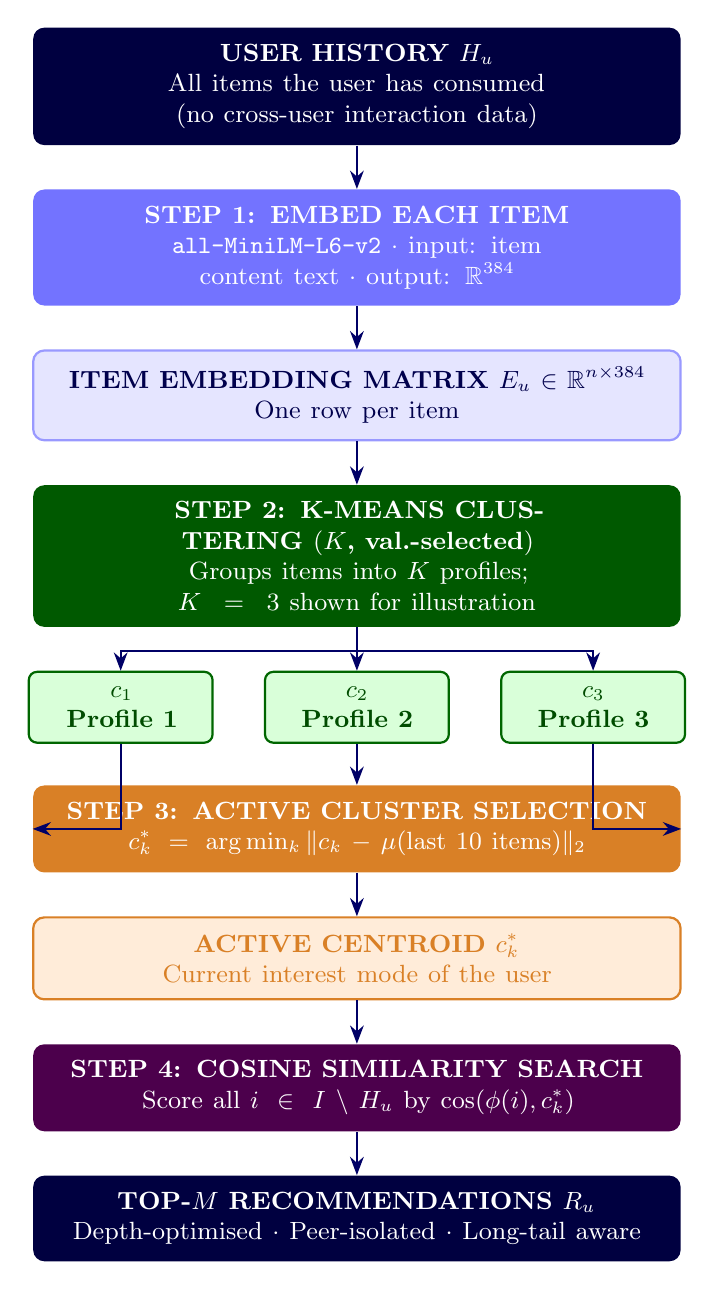
\begin{tikzpicture}[node distance=0.55cm, every node/.style={align=center}]
  \node[navybox]  (hist)   {USER HISTORY $H_u$\\
                             \normalfont\small All items the user has consumed (no cross-user interaction data)};
  \node[bluebox,  below=of hist]  (emb)
        {STEP 1: EMBED EACH ITEM\\
         \normalfont\small \texttt{all-MiniLM-L6-v2} $\cdot$ input: item content text $\cdot$ output: $\mathbb{R}^{384}$};
  \node[lightbox, below=of emb]   (mat)
        {ITEM EMBEDDING MATRIX $E_u \in \mathbb{R}^{n \times 384}$\\ \normalfont\small One row per item};
  \node[greenbox, below=of mat]   (km)
        {STEP 2: K-MEANS CLUSTERING $(K$, val.-selected$)$\\ \normalfont\small Groups items into $K$ profiles; $K=3$ shown for illustration};
  \node[clusterbox, below=of km, xshift=-3.0cm] (c1) {$c_1$\\Profile 1};
  \node[clusterbox, below=of km]                (c2) {$c_2$\\Profile 2};
  \node[clusterbox, below=of km, xshift=+3.0cm] (c3) {$c_3$\\Profile 3};
  \node[brownbox, below=2.0cm of km] (active)
        {STEP 3: ACTIVE CLUSTER SELECTION\\
         \normalfont\small $c_k^* = \arg\min_k \|c_k - \mu(\text{last 10 items})\|_2$};
  \node[warmbox,  below=of active] (ck)
        {ACTIVE CENTROID $c_k^*$\\ \normalfont\small Current interest mode of the user};
  \node[purplebox, below=of ck]   (ann)
        {STEP 4: COSINE SIMILARITY SEARCH\\ \normalfont\small Score all $i \in I \setminus H_u$ by $\cos(\phi(i), c_k^*)$};
  \node[navybox,  below=of ann]   (out)
        {TOP-$M$ RECOMMENDATIONS $R_u$\\
         \normalfont\small Depth-optimised $\cdot$ Peer-isolated $\cdot$ Long-tail aware};
  \draw[arrow] (hist)   -- (emb);
  \draw[arrow] (emb)    -- (mat);
  \draw[arrow] (mat)    -- (km);
  \draw[arrow] (km.south) -- ++(0,-0.3) -| (c1.north);
  \draw[arrow] (km.south) -- ++(0,-0.3) -| (c2.north);
  \draw[arrow] (km.south) -- ++(0,-0.3) -| (c3.north);
  \draw[arrow] (c1.south) |- (active.west);
  \draw[arrow] (c2.south) -- (active.north);
  \draw[arrow] (c3.south) |- (active.east);
  \draw[arrow] (active) -- (ck);
  \draw[arrow] (ck)     -- (ann);
  \draw[arrow] (ann)    -- (out);
\end{tikzpicture}
\caption{Essence recommendation pipeline. No cross-user interaction data is consulted at any stage.}
\label{fig:pipeline}
\end{figure}

\section{Architectural Comparison}
\label{app:comparison}

\begin{table}[H]
\centering
\caption{Architectural comparison: Essence vs.\ prior systems. The primary distinction is not the clustering mechanism, it is the data requirement and what each system is structurally able to score. ``Distinguishes among zero-interaction items'': CF, MIND, and ComiRec derive representations from co-occurrence and so cannot distinguish among items with zero training interactions, since such items receive identical (typically zero) co-occurrence scores; Essence's metadata-derived embeddings differ per item regardless of interaction count. All four systems are empirically evaluated in this work (Section~\ref{sec:results}), which reports the domain-dependent long-tail recovery result in full.}
\label{tab:comparison}
\small
\begin{tabular}{lcccc}
\toprule
\textbf{Property} & \textbf{CF} & \textbf{MIND} & \textbf{ComiRec} & \textbf{Essence} \\
\midrule
Cross-user data required & Yes & Yes & Yes & \textbf{No} \\
Multiple interest profiles & No & Yes & Yes & \textbf{Yes} \\
Gradient-based training required & No & Yes & Yes & \textbf{No} \\
Distinguishes among zero-interaction items & No & No & No & \textbf{Yes} \\
Embedding source & Co-occurrence & Co-occurrence & Co-occurrence & \textbf{Item metadata} \\
\bottomrule
\end{tabular}
\end{table}

\section{Systems Compared: Full Descriptions}
\label{app:systems}

\textbf{Random.} Recommends $M$ items drawn uniformly from the unseen candidate pool; establishes the floor against which all other systems are compared. It draws a single deterministic sample per user from a per-user seed (MD5 hash of the user ID), not an average over repeated draws.

\textbf{Metric aggregation and tie-breaking.} Both Recall@10 and LT-Recall@10 are macro-averaged: the per-user ratio is computed first, then averaged across users (LT-Recall@10 over eligible users only). Ties in the top-$M$ ranking are broken deterministically: by ascending item index for Amazon Books/MovieLens-25M's vectorized scoring, and by embedding-map iteration order for Last.fm-1K's dictionary-based scoring --- both stable and reproducible, though not identical mechanisms.

\textbf{Popularity.} Recommends the $M$ globally most-interacted-with unseen items. Non-personalized; included for comparison but not treated as collaborative filtering.

\textbf{CF (ItemKNN).} Item-based collaborative filtering via cosine similarity over the sparse user-item interaction matrix. No neighbor-count cutoff or shrinkage term is applied: a candidate's score is the cosine-weighted sum over all training items with any co-occurring user, i.e.\ full-neighborhood ($k=\infty$) ItemKNN rather than a truncated top-$k$ variant.

\textbf{Content (Average Embedding).} Mean of all the user's item embeddings, retrieving the $M$ most similar unseen items. Standard content-based filtering without interest decomposition.

\textbf{Essence (validation-selected $K$).} Clusters user history into $K$ centroids ($K=10$ Last.fm-1K/Amazon Books, $K=15$ MovieLens-25M; Section~\ref{sec:framework}), selects the active centroid by Eq.~\ref{eq:active}, retrieves top-$M$ unseen items by Eq.~\ref{eq:reco}.

\textbf{Last-Item.} Recommends the $M$ unseen items most similar, by cosine similarity, to the single most recent item in the user's training history. The simplest possible recency-based retrieval: no averaging, no decay, no clustering.

\textbf{Avg-Last-10.} Recommends the $M$ unseen items most similar to the uniform mean embedding of the user's last 10 training interactions.

\textbf{Recency-Weighted.} Recommends the $M$ unseen items most similar to an exponentially-decay-weighted mean of the user's last 10 training interactions (decay $=0.9$; the most recent item receives weight $\propto 0.9^{0}$, the tenth-most-recent $\propto 0.9^{9}$, renormalized to sum to 1).

\textbf{MIND.} A hand-implemented dynamic-routing multi-interest network, following Li et al.'s original architecture~\cite{li2019} ($K=4$ interest capsules, a bilinear routing matrix shared across capsules, 3 routing iterations, routing logits initialized $b \sim \mathcal{N}(0, 0.01^2)$). An initial implementation zero-initialized $b$, which --- because the shared bilinear matrix makes the pre-routing representation identical across capsules --- guaranteed every capsule updated identically, silently collapsing the model's effective interest count to 1 regardless of the nominal $K$; caught by a synthetic conformance test and fixed before any number reported in this paper was generated.

\textbf{ComiRec (SA).} A hand-implemented self-attentive multi-interest network, following Cen et al.'s original architecture~\cite{cen2020} ($K=4$ interest capsules, per-capsule learned query projections implemented as a single $K$-output linear layer, softmax attention over sequence positions).

\textbf{MIND/ComiRec training.} Both models share the same fixed, untuned training procedure (values taken from the original papers' recommended ranges, not grid-searched): Adam optimizer, learning rate $10^{-3}$, batch size 64, max sequence length 50, up to 50 epochs with early stopping (patience 5) on validation loss over each user's held-out last training interaction. The training objective is a sampled-softmax loss: the positive item's score plus 100 uniform-random negative items' scores (drawn item-uniformly, avoiding the padding index) are passed through a cross-entropy loss against the positive. Item and interest-capsule embeddings are 384-dimensional, matching the shared \texttt{all-MiniLM-L6-v2} embedding space used by every other system.

\section{MIND/ComiRec Multi-Seed Robustness}
\label{app:multiseed}

Table~\ref{tab:multiseed} reports MIND and ComiRec Recall@10 across independent training seeds per dataset (the canonical seed 42 plus 2--3 additional seeds), to check whether the domain-dependence pattern (Section~\ref{sec:domain-dependence}) depends on a single training run. Paired statistical inference for MIND and ComiRec elsewhere in this paper is conditional on each model's canonical (seed-42) training run; this multi-seed analysis evaluates whether the qualitative ordering is robust to initialization, not training-seed variance within the bootstrap itself.

\begin{table}[H]
\centering
\caption{MIND/ComiRec Recall@10 across training seeds. ``Beats Essence'' counts seeds where the baseline's Recall@10 exceeds Essence's own Recall@10 for that dataset (Table~\ref{tab:headline-recall}).}
\label{tab:multiseed}
\small
\begin{tabular}{llccc}
\toprule
\textbf{Dataset (Essence Recall@10)} & \textbf{System} & \textbf{Mean $\pm$ Std} & $n$ & \textbf{Beats Essence} \\
\midrule
\multirow{2}{*}{Last.fm-1K (0.0281)} & MIND & $0.0067 \pm 0.0014$ & 4 & 0/4 \\
 & ComiRec (SA) & $0.0116 \pm 0.0020$ & 4 & 0/4 \\
\midrule
\multirow{2}{*}{Amazon Books (0.0253)} & MIND & $0.0053 \pm 0.0004$ & 4 & 0/4 \\
 & ComiRec (SA) & $0.0064 \pm 0.0007$ & 4 & 0/4 \\
\midrule
\multirow{2}{*}{MovieLens-25M (0.0053)} & MIND & $0.0464 \pm 0.0036$ & 3 & 3/3 \\
 & ComiRec (SA) & $0.0607 \pm 0.0086$ & 3 & 3/3 \\
\bottomrule
\end{tabular}
\end{table}

Essence's Recall@10 here uses its validation-selected $K$ per dataset, not the $K=3$ value used in an earlier revision of this analysis; at $K=3$, ComiRec (SA) beat Essence on 2 of 4 Last.fm-1K seeds, characterized then as not significantly different. At $K=10$, Essence's own Recall@10 rises enough ($0.0119\to0.0281$) that ComiRec no longer beats it on any seed. The domain-dependence pattern itself is not an artifact of a single seed: MIND never outranks Essence on Last.fm-1K or Amazon Books and always outranks Essence on MovieLens-25M, across every seed tested; ComiRec (SA) now shows the same clean pattern on all three datasets rather than being seed-dependent anywhere.

\section{An Additional Collaborative Baseline: BPR-MF}
\label{app:bprmf}

To check that the domain-dependence pattern (Section~\ref{sec:domain-dependence}) does not depend on CF-ItemKNN specifically, we implement BPR-MF~\cite{rendle2009} (Bayesian Personalized Ranking Matrix Factorization): a pairwise-ranking loss over learned latent user/item factors, structurally unlike ItemKNN's neighborhood-based scoring, sharing no code or architecture with it. \textbf{Before trusting any real-dataset number}, we ran a dedicated conformance test on synthetic data --- training loss decreases with training, the model recovers a known latent block structure from synthetic co-occurrence data it was not told about, and a user's single known positive item is correctly recovered near the top of a trivial ranking --- the same discipline that caught the MIND routing bug (Section~\ref{sec:setup}). The conformance test itself needed one correction first (an overly strict pass/fail threshold on the loss-decrease check, not a model bug) before all three checks passed cleanly. Hyperparameters are fixed, not tuned (32 latent factors, learning rate 0.05, L2 regularization 0.01, 30 epochs, seed 42), matching how CF-ItemKNN is treated elsewhere in this paper.

\begin{table}[H]
\centering
\caption{BPR-MF vs.\ Essence, all three datasets (paired bootstrap, raw $p$, not FDR-corrected). Recall@10 differences are significant ($p<0.05$) on all three datasets; LT-Recall@10 differences are significant on Last.fm-1K and Amazon Books but not on MovieLens-25M ($p\approx0.09$).}
\label{tab:bprmf}
\small
\begin{tabular}{lcccc}
\toprule
\textbf{Dataset} & \textbf{Essence R@10} & \textbf{BPR-MF R@10} & \textbf{Essence LT-R@10} & \textbf{BPR-MF LT-R@10} \\
\midrule
Last.fm-1K & 0.0281 & 0.0005 & 0.0142 & 0.0000 \\
Amazon Books & 0.0253 & 0.0015 & 0.0207 & 0.0000 \\
MovieLens-25M & 0.0053 & 0.0647 & 0.0030 & 0.0000 \\
\bottomrule
\end{tabular}
\end{table}

The result replicates the domain-dependence pattern exactly. Where collaborative signal is weak, Essence beats BPR-MF (raw $p<0.05$, uncorrected; Last.fm-1K: $d=+0.296$; Amazon Books: $d=+0.261$). Where collaborative signal is strong, Essence loses to it (raw $p<0.05$, uncorrected; MovieLens-25M: $d=-0.518$, BPR-MF ranking immediately behind CF-ItemKNN and ComiRec among all systems tested there). BPR-MF's own LT-Recall@10 is $0.0000$ on all three datasets, including MovieLens-25M where it wins on Recall@10 --- consistent with the paper's broader observation that strong aggregate collaborative performance does not translate into long-tail recovery (Section~\ref{sec:discussion}).

BPR-MF's significance tests are reported as raw $p$-values rather than folded into one of this paper's existing FDR-corrected families (Section~\ref{sec:stats-methodology}): BPR-MF was added as an ad hoc, late-stage robustness probe, not part of the pre-specified evaluation design those families were built from, so it is disclosed standalone rather than artificially forced into a family it was never planned alongside. BPR-MF is an untuned, exploratory robustness baseline. Its strong MovieLens-25M performance reproduces the direction of the ItemKNN result (Section~\ref{sec:limitations} discusses ItemKNN's own separate tuning check), but its performance on the other two datasets may be understated by the fixed configuration used here.

\section{Overnight Robustness-Check Summary}
\label{app:robustness}

Table~\ref{tab:robustness} summarizes the four additional robustness checks referenced in Section~\ref{sec:limitations}: rating-threshold sensitivity, a global-timestamp-cutoff split, multi-seed resampling, and validation-based ItemKNN hyperparameter tuning. Sample-size changes matter for reading these numbers: the global-cutoff and rating-threshold checks each exclude some users, most severely for MovieLens-25M under the global cutoff (98.6\% stranded), so those rows are more a test of the split protocol itself than a like-for-like comparison to the canonical numbers.

\begin{table}[H]
\centering
\caption{Overnight robustness-check summary. ``Essence R@10'' compares the canonical per-user-split, seed-42 Recall@10 to each check's result; ``CF R@10'' (tuning row only) compares CF-ItemKNN's own Recall@10, since that is what was tuned, not Essence.}
\label{tab:robustness}
\small
\begin{tabular}{lll}
\toprule
\textbf{Check} & \textbf{Sample size / users affected} & \textbf{Recall@10 outcome} \\
\midrule
Rating-threshold ($\geq 4$) & Amazon: 1{,}602/2{,}000 (20\% dropped); & Amazon: $0.0253\to0.0300$; \\
 & MovieLens: 1{,}432/2{,}000 (28\% dropped) & MovieLens: $0.0053\to0.0060$ \\
\midrule
Multi-seed resampling (2 extra seeds) & Amazon/MovieLens: 2{,}000/2{,}000 each seed & Amazon: $0.0253\to0.0256$--$0.0258$; \\
 & (different users, same count) & MovieLens: $0.0053\to0.0056$--$0.0066$ \\
\midrule
Global-timestamp cutoff & Last.fm-1K: 60/99 (39\% stranded); & Last.fm-1K: $0.0281\to0.0032$; \\
 & Amazon: 1{,}124/2{,}000 (44\%); & Amazon: $0.0253\to0.0164$; \\
 & MovieLens: 28/2{,}000 (98.6\%) & MovieLens: $0.0053\to0.0014$ \\
\midrule
ItemKNN validation-based tuning & All users, all three datasets & CF R@10: Last.fm $0.0018\to0.0005$ ($-69\%$); \\
 & (no exclusions; CF-ItemKNN retuned) & CF R@10: Amazon $0.0031\to0.0062$ ($+98\%$); \\
 & & CF R@10: MovieLens $0.0850\to0.0850$ ($0\%$) \\
\bottomrule
\end{tabular}
\end{table}

\section{Claim-Reversal: How the Apparent Conclusion Shifted}
\label{app:claimreversal}

Table~\ref{tab:claimreversal} reconstructs how the headline conclusion this paper would have supported changed as evaluation stages were added, using only numbers already reported above (Table~\ref{tab:systems}, Table~\ref{tab:domain-dependence}, Section~\ref{sec:limitations-findings}) --- no new comparisons are run for this table.

\begin{table}[H]
\centering
\caption{How the apparent headline conclusion shifts as evaluation stages are added, using only already-reported numbers.}
\label{tab:claimreversal}
\scriptsize
\begin{tabular}{p{2.1cm}p{4.3cm}p{5.4cm}}
\toprule
\textbf{Stage} & \textbf{Evidence at this stage} & \textbf{Apparent conclusion} \\
\midrule
1.\ Naive baselines & Amazon: Essence $0.0253$ vs.\ CF $0.0031$, Popularity $0.0021$ & Essence clearly beats CF and popularity. \\
\midrule
2.\ + recency baselines & Amazon: Last-Item $0.0311$, Recency-Weighted $0.0260$ exceed Essence's $0.0253$; Avg-Last-10 ($0.0235$) does not & Essence's edge over CF was partly just recency, not clustering. \\
\midrule
3.\ + bootstrap/FDR & Essence loses \emph{significantly} to Last-Item ($d=-0.058$) on Amazon but is not significantly different from Recency-Weighted ($d=-0.009$); still beats CF/Popularity/both neural baselines significantly & Essence's supported value is beating CF/popularity/neural baselines; only Last-Item remains a significant loss. \\
\midrule
4.\ + third dataset & Essence ranks 8th/10 on MovieLens ($0.0053$ vs.\ CF's $0.0850$), $d$ down to $-0.550$ & Whether Essence's advantage holds is associated with domain CF/popularity strength, not shown to be predictive of it (Section~\ref{sec:domain-dependence}). \\
\midrule
5.\ + clustering-mechanism test & Essence never significantly beats Recency-Weighted in any silhouette stratum; of 16 clean comparisons, only 1 is a significant loss (MovieLens high stratum, LT-Recall@10, $d=-0.092$) & Clustering itself, isolated from recency weighting, is not empirically supported as the source of Essence's advantage; the case that it actively hurts is narrow, not broad. \\
\midrule
6.\ + validation-selected $K$ (replacing fixed $K{=}3$) & Essence's own numbers rise on Last.fm-1K/Amazon Books at the new $K$ ($0.0119\to0.0281$; $0.0221\to0.0253$), moving it from 5th/4th to 2nd/3rd; stratification's significant-loss count drops from 6 of 17 (at $K{=}3$) to 1 of 16 & Fixing $K=3$ without validating it understated Essence's standing on two of three datasets and overstated how often clustering actively hurts specific users; MovieLens-25M is essentially unchanged. \\
\bottomrule
\end{tabular}
\end{table}

Each stage narrows the claim rather than overturning the last: from ``clustering beats collaborative filtering'' to ``recency-aware retrieval mostly matches or beats collaborative filtering, clustering's own contribution is domain-dependent, and neither the case for clustering nor the case against it survives an untuned $K$ without narrowing further.''

\section{Active Cluster Selection Ablation}
\label{app:ablation}

We test the recency-based active-cluster-selection mechanism (Section~\ref{sec:framework}) against an alternative: selecting the active centroid using the mean embedding of the user's entire training history rather than the most recent $r=10$ interactions, now on all three datasets at their validation-selected $K$.

\begin{table}[H]
\centering
\caption{Active cluster selection ablation, all three datasets at their validation-selected $K$ (chronological split, $M=10$).}
\label{tab:ablation}
\small
\begin{tabular}{llccc}
\toprule
\textbf{Dataset} & \textbf{Variant} & \textbf{Recall@10} & \textbf{LT-Recall@10} & \textbf{LT / Content} \\
\midrule
\multirow{3}{*}{Last.fm-1K ($K{=}10$)}
 & Essence (recency, $r{=}10$) & 0.0281 & 0.0142 & $4.84\times$ \\
 & Essence (mean-select) & 0.0016 & 0.0005 & $0.16\times$ \\
 & Content (reference) & 0.0038 & 0.0029 & $1.0\times$ \\
\midrule
\multirow{3}{*}{Amazon Books ($K{=}10$)}
 & Essence (recency, $r{=}10$) & 0.0253 & 0.0207 & $1.67\times$ \\
 & Essence (mean-select) & 0.0195 & 0.0118 & $0.95\times$ \\
 & Content (reference) & 0.0173 & 0.0124 & $1.0\times$ \\
\midrule
\multirow{3}{*}{MovieLens-25M ($K{=}15$)}
 & Essence (recency, $r{=}10$) & 0.0053 & 0.0030 & $1.46\times$ \\
 & Essence (mean-select) & 0.0044 & 0.0037 & $1.83\times$ \\
 & Content (reference) & 0.0043 & 0.0020 & $1.0\times$ \\
\bottomrule
\end{tabular}
\end{table}

On Last.fm-1K, mean-select performs below even the Content baseline on long-tail recall (LT/Content, $4.84\times$ in recency-select's favor), consistent with the mechanism collapsing toward Content. On Amazon Books, the same pattern holds but less extremely: mean-select stays above Content rather than collapsing below it. On MovieLens-25M the result is mixed: recency-select leads on Recall@10 but mean-select leads on LT-Recall@10. No significance testing has been run on these differences. Recency-based selection is retained as Essence's default on the strength of the Last.fm-1K/Amazon Books results; MovieLens-25M's mixed result is reported rather than smoothed over.

\section{Effect of User-Authored Review Embeddings (Amazon Books)}
\label{app:pass2}

As a secondary experiment, we tested whether building user taste profiles from review text (first-person language describing a user's reaction to consumed items) rather than item metadata changes Essence's relative performance.

\begin{table}[H]
\centering
\caption{Amazon Books: metadata embeddings (Pass 1) vs.\ user-review embeddings (Pass 2). Pass 2 builds taste profiles from the user's own review text; candidates are scored using metadata embeddings. This secondary experiment uses $K=3$ throughout and has not been re-run at Essence's validation-selected $K=10$; reported as a fixed-$K$ diagnostic, not a headline result.}
\label{tab:amazon_pass2}
\small
\begin{tabular}{llccc}
\toprule
\textbf{Pass} & \textbf{System} & \textbf{Recall@10} & \textbf{LT-Recall@10} & \textbf{LT / Content} \\
\midrule
\multirow{3}{*}{Pass 1 (metadata)}
  & CF (ItemKNN) & 0.0031 & 0.0137 & --- \\
  & Content (Avg) & 0.0173 & 0.0124 & $1.0\times$ \\
  & Essence ($K=3$) & 0.0221 & 0.0197 & $1.59\times$ \\
\midrule
\multirow{3}{*}{Pass 2 (user review)}
  & CF (ItemKNN) & 0.0031 & 0.0137 & --- \\
  & Content (Avg) & 0.0027 & 0.0012 & $1.0\times$ \\
  & Essence ($K=3$) & 0.0041 & 0.0034 & $2.83\times$ \\
\bottomrule
\end{tabular}
\end{table}

Absolute recall degrades substantially in Pass 2. Two factors likely contribute: an input-distribution mismatch (taste profiles are built from review-text embeddings while candidates are still scored using metadata embeddings, and although both come from the same encoder, review text and item metadata occupy different regions of the shared embedding space), and review text being a noisier input than structured metadata (a review may describe shipping conditions or personal circumstances unrelated to the item's content). Essence's relative advantage over Content persists in Pass 2 ($2.83\times$ vs.\ $1.59\times$ in Pass 1, both above parity), suggesting the $K$-means clustering mechanism extracts usable interest structure even under degraded input quality. The absolute recall values in Pass 2 are low enough that this comparison carries limited statistical weight; we treat it as a directional observation motivating embedding-input-curation as future work.

\section{Full Statistical-Family Reasoning}
\label{app:fdr}

The Last.fm-1K/Amazon Books baseline comparison (Essence vs.\ each of the nine other systems, per dataset, per metric; 36 comparisons) and the multimodality-stratification test (Essence vs.\ Recency-Weighted, stratified by each user's own per-history silhouette score into low/medium/high clustering-quality tertiles, per dataset, per metric; up to 18 comparisons) are corrected together as a single Benjamini--Hochberg family, nominally 54 comparisons, since pooling changes no comparison's significance verdict relative to correcting them separately (verified directly). In practice the family is 52 comparisons at the validation-selected $K$ and 53 at an earlier $K=3$ version of this analysis, not 54: one or two stratification cells are \emph{degenerate} --- every user in that stratum/metric cell scores exactly $0$ on \emph{both} Essence and Recency-Weighted (most often a low- or medium-silhouette stratum on the smaller LT-Recall@10 subsets), giving zero variance in the paired bootstrap difference. The standard two-sided $p$-value formula, $p = 2\min(\hat{P}(\text{diff}{>}0), 1-\hat{P}(\text{diff}{>}0))$, is undefined when every resample gives diff${}={}0$ exactly: naively applying it returns $\hat{P}(\text{diff}{>}0)=0$ and hence $p=0$, reading as maximally significant when in fact there is no difference to detect (Cohen's $d$ is also undefined here, $0/0$). We exclude these cells from the pooled family rather than count them as evidence; this correction applies retroactively to an earlier $K=3$ version of this analysis, which counted one such cell (Last.fm-1K, low-silhouette stratum, LT-Recall@10, $n=32$, all values $0$) as significant. The MovieLens-25M baseline comparison (18 comparisons) is corrected separately: it tests the same underlying question as the family above but was not included in the pooling-invariance check performed on it. The decile-level cold-start analysis (Essence, and separately each recency-only baseline, vs.\ CF-ItemKNN, restricted to the rarest-item deciles) is corrected as its own family: it asks a narrower, mechanistically distinct question, isolating a single structural property of CF (zero co-occurrence signal for zero-training-interaction items) rather than asking about aggregate performance, and was decided as a separate question before being run --- not a post-hoc re-slicing of the primary comparison chosen because a pooled result was inconvenient.

\section{Extended Discussion}
\label{app:discussion}

\textbf{Mechanism.} Item-based CF records zero long-tail recall on the sparsest dataset, Last.fm-1K, under deterministic ranking; on the denser Amazon Books it surfaces some low-interaction items but pays a large cost to overall recall ($0.0031$, near the bottom of the field). MovieLens-25M is the case where this popularity-feedback dynamic would run at full strength in the other direction, consistent with though not directly measured by this evaluation: CF's Recall@10 ($0.0850$) is the highest value recorded anywhere in this study, and Popularity itself ranks 3rd of 10 overall ($0.0517$), yet CF's LT-Recall@10 ($0.0037$) remains far below its own overall Recall@10.

\textbf{Deployment and privacy.} The absolute recall values reported here (roughly $0.005$--$0.03$ under full-catalog evaluation) should be read in light of deployment context: Essence is not proposed as a replacement for a primary, CF-driven feed. On Amazon Books and Last.fm-1K it is better understood as a specialized retrieval path for a dedicated discovery surface (e.g.\ a ``more like this'' interface) where the goal is surfacing items dissimilar from what population-level signals would recommend; this framing does not hold on MovieLens-25M. Separately, because Essence consults no cross-user interaction data at any stage, it remains deployable in settings where CF is not viable at all --- privacy-regulated environments, on-device recommendation without server-side interaction logs, federated settings, and cold-start contexts where no population-level interaction graph exists yet --- a direct architectural consequence, independent of whether Essence wins on a given domain's aggregate metrics.

\section{Extended Limitations and Future Work}
\label{app:limitations}

\textbf{Filter bubble risk.} Peer-isolation removes the serendipity cross-user signals can provide; whether repeated centroid queries cause semantic narrowing is an open empirical question. \textbf{Embedding input curation.} Appendix~\ref{app:pass2} shows noisy embedding inputs degrade performance; the quality of what enters the embedding determines the quality of what Essence can find, and automated curation of embedding input text is a direct practical extension. \textbf{Audio-based embeddings.} Current embeddings derive from item metadata text only; for music, incorporating audio-based representations (sonic texture, timbre, rhythm, harmonic structure) would more precisely model the latent acoustic fingerprint underlying individual taste, and is the primary planned extension of Essence. \textbf{Cross-space embedding alignment.} Appendix~\ref{app:pass2}'s results suggest that aligning review-text and metadata input distributions within the shared embedding space (via contrastive training or a learned projection layer) could unlock the full signal of user-authored representations while maintaining retrieval coherence. \textbf{Active cluster selection.} The recency-based heuristic is simple by design; a learned selection mechanism could improve session-aware accuracy without requiring cross-user training.

\newpage
\section*{NeurIPS Paper Checklist}

\begin{enumerate}

\item {\bf Claims}
    \item[] Question: Do the main claims made in the abstract and introduction accurately reflect the paper's contributions and scope?
    \item[] Answer: \answerYes{}
    \item[] Justification: The abstract and introduction state the domain-dependent, mixed result directly (the Amazon Books/Last.fm-1K wins and non-significant results, the MovieLens-25M loss, and the clustering-mechanism null result from the stratification test) rather than only the favorable case; the body (Sections~\ref{sec:results}--\ref{sec:limitations}) matches this framing throughout.

\item {\bf Limitations}
    \item[] Question: Does the paper discuss the limitations of the work performed by the authors?
    \item[] Answer: \answerYes{}
    \item[] Justification: Section~\ref{sec:limitations-findings} and Section~\ref{sec:limitations} discuss scale, the $K$-selection procedure's own anchoring caveat, the hand-implemented (not pre-trained) status of MIND/ComiRec, and the post-hoc nature of the domain-dependence characterization; Appendix~\ref{app:limitations} extends this further.

\item {\bf Theory assumptions and proofs}
    \item[] Question: For each theoretical result, does the paper provide the full set of assumptions and a complete (and correct) proof?
    \item[] Answer: \answerNA{}
    \item[] Justification: This is an empirical paper; it contains no theorems or proofs.

\item {\bf Experimental result reproducibility}
    \item[] Question: Does the paper fully disclose all the information needed to reproduce the main experimental results?
    \item[] Answer: \answerYes{}
    \item[] Justification: Section~\ref{sec:setup} and Appendix~\ref{app:systems} specify all datasets, splits (chronological, 80/20 per user, seed 42), hyperparameters ($K$ validation-selected per dataset via the procedure in Section~\ref{sec:framework}: $K=10$/$10$/$15$; $r=10$, decay $=0.9$, $M=10$), the embedding model, and every baseline's exact query construction; Appendix~\ref{app:fdr} specifies the significance-testing methodology in full. Section~\ref{sec:framework} additionally documents the $K$-means configuration (\texttt{k-means++}, \texttt{n\_init=10}, \texttt{random\_state=42}) and the minimum per-user training-history size on each dataset, confirming the fallback for users with fewer than $K$ items was not triggered at any validated $K$. Appendix~\ref{app:bprmf} specifies the additional BPR-MF baseline's hyperparameters and conformance-testing procedure in full.

\item {\bf Open access to data and code}
    \item[] Question: Does the paper provide open access to the data and code, with sufficient instructions to faithfully reproduce the main experimental results?
    \item[] Answer: \answerYes{}
    \item[] Justification: Anonymized code and data are available at \url{https://anonymous.4open.science/r/essence-5B7B/README.md}, including full reproduction instructions for every analysis reported in this paper. The data included is filtered, processed interaction-level subsets, not the full raw datasets; see the Licenses item below for exactly what this includes and an unresolved MovieLens-25M redistribution caveat. The repository will be de-anonymized and linked to its permanent location upon deanonymization.

\item {\bf Experimental setting/details}
    \item[] Question: Does the paper specify all the training and test details necessary to understand the results?
    \item[] Answer: \answerYes{}
    \item[] Justification: See Section~\ref{sec:setup} and Appendix~\ref{app:systems}: chronological train/test split, all baseline query constructions, and MIND/ComiRec architecture hyperparameters are specified; Section~\ref{sec:framework} specifies the $K$-means configuration and the minimum per-user training-history size relative to each dataset's validated $K$.

\item {\bf Experiment statistical significance}
    \item[] Question: Does the paper report error bars suitably and correctly defined or other appropriate information about the statistical significance of the experiments?
    \item[] Answer: \answerYes{}
    \item[] Justification: This is a central contribution of the paper (Section~\ref{sec:stats-methodology}, Appendix~\ref{app:fdr}): all primary baseline and stratification comparisons use a paired bootstrap significance test ($10{,}000$ resamples) with reported mean difference, 95\% CI, and Cohen's $d$; Benjamini--Hochberg FDR correction is applied within separately defined comparison families; BCa resampling cross-checks every raw-significant result.

\item {\bf Experiments compute resources}
    \item[] Question: For each experiment, does the paper provide sufficient information on the computer resources needed to reproduce the experiments?
    \item[] Answer: \answerYes{}
    \item[] Justification: All experiments ran on a single consumer laptop (Apple M4 Pro, macOS, no CUDA GPU); MIND/ComiRec use Apple's MPS backend when available, CPU otherwise. Essence's per-user cost is dominated by the $K$-means fit (mean $\approx$10ms/user, both Last.fm-1K and Amazon Books), not candidate scoring ($<2$ms/user regardless of catalog size, a single matrix-vector product); full per-user inference ranges from $\approx$1ms (CF-ItemKNN) to $\approx$70ms (Essence, Last.fm-1K). The full downstream chain (evaluation, paired bootstrap, FDR, decile analysis, silhouette stratification, active-cluster ablation) at each dataset's validation-selected $K$ took 168.6s (Last.fm-1K), 1{,}057.1s (Amazon Books), and 473.6s (MovieLens-25M) wall-clock, single-threaded, no parallelization across datasets. No GPU cluster or specialized hardware is required to reproduce any result in this paper.

\item {\bf Code of ethics}
    \item[] Question: Does the research conducted in the paper conform, in every respect, with the NeurIPS Code of Ethics?
    \item[] Answer: \answerYes{}
    \item[] Justification: This work evaluates recommendation algorithms on standard, publicly available, de-identified interaction datasets (Last.fm-1K, Amazon Reviews, MovieLens-25M); it involves no human-subjects research, no crowdsourcing, and no release of models with elevated misuse risk.

\item {\bf Broader impacts}
    \item[] Question: Does the paper discuss both potential positive societal impacts and negative societal impacts of the work performed?
    \item[] Answer: \answerYes{}
    \item[] Justification: Section~\ref{sec:discussion} includes a dedicated Broader Impact paragraph discussing the potential positive impact (personalization without a pooled cross-user interaction graph, relevant to privacy-regulated and on-device deployment) and potential risks (filter-bubble/semantic-narrowing effects, and possible degraded quality for users with sparse or atypical histories).

\item {\bf Safeguards}
    \item[] Question: Does the paper describe safeguards for responsible release of data or models with high misuse risk?
    \item[] Answer: \answerNA{}
    \item[] Justification: The paper releases no generative models, scraped image data, or other assets with elevated misuse potential.

\item {\bf Licenses for existing assets}
    \item[] Question: Are the creators or original owners of assets used in the paper properly credited and are license and terms of use explicitly mentioned?
    \item[] Answer: \answerYes{}
    \item[] Justification: All datasets and models used are credited above (Section~\ref{sec:setup}) and their license terms, as verified against each source's own published terms, are: \emph{Last.fm-1K} --- distributed with permission of Last.fm for non-commercial use only, per the dataset's official page; commercial use requires contacting Last.fm directly. \emph{MovieLens-25M} --- GroupLens's usage license prohibits redistribution without separate permission and prohibits commercial or revenue-bearing use without permission; research use is permitted with citation and no claim of University of Minnesota endorsement. \emph{Amazon Reviews 2023 (Books 5-core)}~\cite{hou2024} --- no explicit license file or tag is published on the dataset's official site or Hugging Face card as of this writing; the only stated usage term is citation of the originating paper, so redistribution/commercial terms cannot be independently verified and none are claimed here. \texttt{all-MiniLM-L6-v2} --- Apache~2.0 (permissive, commercial use allowed), per its Hugging Face model card. \emph{TMDb API} --- used under TMDb's standard attribution requirement: this paper uses the TMDb API but is not endorsed or certified by TMDb. The accompanying repository includes filtered, chronologically-split, interaction-level subsets derived from each dataset (user/item identifiers, ratings or plays, timestamps, and for Amazon Books and MovieLens-25M, associated review/metadata text) for reproducibility --- not the full raw datasets, but more than aggregate statistics alone. For MovieLens-25M specifically, this is in tension with GroupLens's redistribution restriction quoted above; separate permission has not been sought. This is disclosed here directly rather than elided.

\item {\bf New assets}
    \item[] Question: Are new assets introduced in the paper well documented and is the documentation provided alongside the assets?
    \item[] Answer: \answerYes{}
    \item[] Justification: The from-scratch MIND/ComiRec implementations and the processed, interaction-level dataset subsets described in the Licenses item above are new assets; the anonymized repository (see the Open Access item above) includes both, along with reproduction instructions for every analysis reported in this paper. See the Licenses item for the MovieLens-25M redistribution caveat.

\item {\bf Crowdsourcing and research with human subjects}
    \item[] Question: For crowdsourcing experiments and research with human subjects, does the paper include the full text of instructions given to participants and details about compensation?
    \item[] Answer: \answerNA{}
    \item[] Justification: This paper involves no crowdsourcing or human-subjects research; all data consists of pre-existing, publicly released interaction logs.

\item {\bf Institutional review board (IRB) approvals or equivalent for research with human subjects}
    \item[] Question: Does the paper describe potential risks incurred by study participants and whether IRB approval was obtained?
    \item[] Answer: \answerNA{}
    \item[] Justification: No human-subjects research was conducted; no IRB review was required.

\item {\bf Declaration of LLM usage}
    \item[] Question: Does the paper describe the usage of LLMs if it is an important, original, or non-standard component of the core methods in this research?
    \item[] Answer: \answerYes{}
    \item[] Justification: No LLM is a component of any method evaluated in this paper --- Essence, the collaborative-filtering and content-based baselines, MIND, ComiRec, and the significance-testing methodology (paired bootstrap, Benjamini--Hochberg FDR, BCa) are all standard, non-LLM techniques. Consistent with this checklist item's own exemption for ``writing, editing, or formatting,'' AI assistance was used as a development and verification tool during implementation --- including catching a symmetry-breaking initialization bug in our own MIND implementation (Section 4) and flagging several numeric and framing inconsistencies during manuscript preparation, each independently reviewed and confirmed against source data by the authors before being reported. No experimental result, statistical test, or claim in this paper was generated or accepted without direct author verification.

\end{enumerate}

\end{document}
